\documentclass[11pt,final,journal,a4paper,towside,towcolumn]{IEEEtran}
%\usepackage{cite}
\usepackage{graphicx}
\usepackage[utf8]{inputenc}
\usepackage[nolist]{acronym}
\usepackage{multirow}
\usepackage[table,xcdraw]{xcolor}

\begin{document}
\begin{acronym}
	\acro{NEAT}{NeuroEvolution of Augmenting Topologies}
	\acro{KI}{Künstliche Intelligenz}
\end{acronym}
	
%\title{Abschlussbericht des Team $m^2$ zu dem \\Projektpraktikum Robotik und Automation:\\Künstliche Intelligenz}
\title{Projektpraktikum Robotik und Automation:\\Künstliche Intelligenz}
\author{Team $m^2$: Marius Krusen und F. J. Michael Werner}
\maketitle

\section{Aufgabenstellung}
\IEEEPARstart{Z}{iel} des Projektpraktikums ist es, eine funktionsfähige  \ac{KI} für das Spiel rAIcer zu entwickeln. In dem Spiel können bis zu drei Spieler jeweils eine Figur über mehrere Runden auf einer Rundstrecke steuern. Die Figuren werden nur durch "Kraftimpulse" in den Richtungen oben, unten, links und rechts gesteuert. In einem abschließenden Turnier, soll die \ac{KI} in der Lage sein, auf bekannten sowie unbekannten Strecken gegen \acp{KI} anderer Teams anzutreten.

\section{Lösungsansatz}
Das Team $m^2$ verwendet für die Entwicklung der \ac{KI} den \ac{NEAT}-Algorithmus. Weiterhin wird das gegebene Problem darauf reduziert, dass die \ac{KI} eine Folge von Kontrollpunkten auf der Strecke abfahren muss. Für die Berechnung der Kontrollpunkte ist eine Streckenerkennung notwendig. Für die Eingabe, der durch den \ac{NEAT}-Algorithmus generierten neuronalen Netze, werden Merkmale berechnet, die unter anderem auf den Kontrollpunkten und der Position der Figur basieren. Die einzelnen Elemente des Lösungsansatzes werden nachfolgend im Detail vorgestellt.
\subsection{NEAT}
In der Neuroevolution werden Neuronale Netze mit Hilfe von genetischen Algorithmen generiert. In \cite{stanley:gecco02-efficient} stellen Stanley et al. \ac{NEAT} vor, der die Besonderheit hat, dass neben den Kantengewichten und Schwellenwerten, auch die Topologie des Netzes entwickelt wird.
Die zentralen Bausteine des Algorithmus sind:
\begin{itemize}
\item Darstellung eines Netzes als Genom	
\item Verwendung von Historie-Markern
\item Verwendung von Spezies
\item Minimierung der Dimensionalität
\end{itemize}
In jeder Generation liegt eine Menge von Genomen (Population) vor. Durch eine Fitnessfunktion, wird die Performance der einzelnen Genome bestimmt. Anschließend werden basierend auf den stärkeren Genomen mithilfe von Mutation und Kreuzungen neue Genome für die nächste Generation erzeugt. 
Für die Implementierung des Projektes wurde das Python-Package NEAT-Python \cite{python-neat} verwendet.
 
%\subsubsection*{Genetische Darstellung und Mutation}
%Jedes Genom besteht aus einer Liste von Kanten-Genen. Diese referieren jeweils auf zwei Knoten-Gene, die deren Eingangs- und Ausgangsknoten darstellen. Des Weiteren enthalten die Kanten-Gene Informationen über ihre Kantengewichte, ein Aktivierungsbit und eine Innovationsnummer. 

%Mutationen in \ac{NEAT} können die Kantengewichte und die Netzstruktur verändern. Die Mutation der Kantengewichte erfolgt über Entscheidung, basierend auf Wahrscheinlichkeiten, ob ein Knoten mutiert oder nicht. Die Mutation der Struktur kann auf zwei Weisen erfolgen. Zum einen kann ein einzelnes Kanten-Gen zwischen zwei bisher nicht verbunden Knoten-Genen hinzugefügt werden, zum anderen kann ein Kanten-Gen durch zwei neue Kanten-Gene und ein neues Knoten-Gen ersetzt werden. Das alte Kanten-Gen wird dabei deaktiviert. Dadurch wird ein neuer Knoten in die Netzstruktur eingefügt.

%\subsubsection*{Historie-Marker und Kreuzungen}
%Für die Kreuzung zweier Genome muss überprüft werden, welche Gene übereinstimmen. Dafür wird bei jedem neuen Gen eine globale Innovationsnummer erhöht und diesem Gen zugewiesen. Zwei Gene, die den gleichen historischen Ursprung haben, also eine gleiche Innovationsnummer besitzen, repräsentieren die gleiche Struktur. Während der Kreuzung kann so leicht bestimmt werden, welche Gene in beiden Elterngenomen vorliegen und übernommen werden können. Gene, die nicht in beiden Elterngenomen vorkommen, werden von dem Elterngenome mit dem höheren Fitnesswert vererbt.

%\subsubsection*{Spezies}
%Durch das Hinzufügen einer neuen Struktur wird die Fitness anfänglich reduziert. Um eine neue Innovation zu schützen und ihr Zeit zur Optimierung zu geben, unterteilt \ac{NEAT} die Population in mehrere Spezies. Eine neue Innovation konkurriert erst mit den Genomen in der jeweiligen Spezies. Erst nach eine gewissen Zeit, wird eine Auslöschung durch einen Vergleich mit der restlichen Population möglich. Die Einteilung der Population in Spezies erfolgt durch die Berechnung einer Distanz zwischen zwei Genomen $\delta$:
%\begin{equation}
%\delta=\frac{c_1E}{N} + \frac{c_2D}{N} + c_3\cdot \overline{W},
%\end{equation}
%mit der Anzahl überflüssiger Gene $E$, die Anzahl verschiedener Gene $D$ und der durchschnittlichen Differenz der Kantengewichte übereinstimmender Gene $\overline{W}$. Die Koeffizienten $c_1, c_2, c_3$ dienen zur Gewichtung der Faktoren und $N$, die Anzahl an Genen in dem größeren Genom, dient zu Normalisierung der Distanz. Jedes Genom wird mit einem zufällig ausgewählten Genom einer Spezies verglichen. Wird ein Schwellenwert $\delta_t$ unterschritten, wird das Genom der Spezies hinzugefügt.

%\subsubsection*{Minimierung der Dimensionalität}
%\ac{NEAT} sieht vor, dass die anfängliche Population aus Netzen besteht, die keine verdeckten Knoten und keine Kanten hat. Dadurch das Innovationen geschützt werden, können somit möglichst kleine Netze generiert werden, da nur neue Strukturen hinzugefügt werden, wenn sie im Sinne der Fitnessfunktion Verbesserungen einbringen.
%Allerdings ermöglicht die \ac{NEAT}-Implementierung aus \cite{python-neat}, dass auch mit nicht leeren Neuronalen Netzen begonnen werden kann. Diese Funktion wurde auch in unseren Experimenten verwendet.

\subsection{Streckenerkennung und Kontrollpunkte}
Die Streckenerkennung und die Berechnung einer Art Ideallinie oder Leitlinie, die durch eine endliche Anzahl an Kontrollpunkten repräsentiert wird, beruht im Wesentlichen auf zwei Algorithmen. Mit Hilfe der Watershed-Algorithmus wird zunächst eine grobe Leitlinie erzeugt, die einen "sicheren" Verlauf entlang der Mitte der Strecke liefert. Anschließend wird diese Leitlinie durch Verwendung eines Snake-Algorithmus, der überflüssige Richtungsänderungen eliminiert und insgesamt einen kürzeren, glatteren Kurvenverlauf erzeugt, verbessert.

\subsubsection{Watershed-Algorithmus}
Um zu Beginn überhaupt ein eindeutiges, klares Bild der Strecke zu bekommen, wird ein einfaches Schwellenwertverfahren eingesetzt, dass alle Pixel mit einem Grauwert unter 10 als schwarz und alle anderen als weiß interpretiert. Um kleine Artefakte, wie den schwarzen Rand der Figur, zu entfernen wird das resultierende Binärbild durch ein \emph{Opening} (eine Erosion gefolgt von einer Dilatation) gefiltert.
Anschließend werden mit Hilfe von OpenCV \cite{opencv} die Konturen der Strecke gefunden, um den inneren Rand der Strecke vom äußeren Rand und möglichen Hindernissen auf der Strecke zu unterscheiden. Der innere Rand wird mit Label 1 markiert, der äußere Rand und Hindernisse mit Label 2. Die eigentliche Strecke erhält kein Label. Auf Basis dieser Labels wird der Watershed-Algorithmus auf einem leeren, einfarbigen Bild ausgeführt. Der Algorithmus wird nicht auf das Bild der Strecke angewendet, da ja nicht die Ränder der Strecke, sondern die Mitte der Strecke gefunden werden soll. Durch das \emph{Fluten} des Bildes ausgehend von den Labels entsteht genau in der Mitte der Strecke eine Linie, an der Label 1 und Label 2 aufeinander treffen. Dies ist die erste grobe Leitlinie, von der in regelmäßigen Abständen ein Punkt als Kontrollpunkt für die weitere Berechnung ausgewählt wird (Bild \ref{fig-watershed}).
\begin{figure}
	\centering
	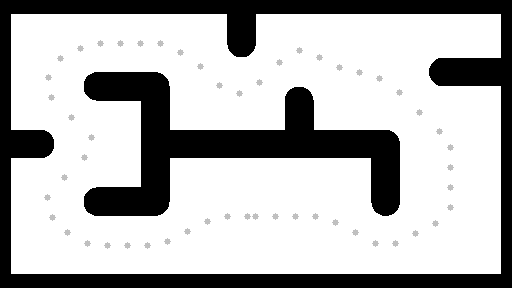
\includegraphics[width=\columnwidth]{watershed_result.png}
	\caption[Watershed-Ergebnis]{Die resultierenden Kontrollpunkte nach Anwendung des Watershed-Algorithmus}
	\label{fig-watershed}
\end{figure}

\subsubsection{Snake-Algorithmus}
Bevor der Snake-Algorithmus die Leitlinie glättet, wird der Rand der Strecke (innen, außen und Hindernisse) um den Radius der Figur dilatiert, um zu verhindern, dass der Algorithmus Kontrollpunkte liefert, die für die Figur gar nicht erreichbar sind.
Der Snake-Algorithmus (auch \emph{Aktive Kontur} genannt) beruht auf einem zu minimierendem Energieterm, der sich normalerweise aus drei einzelnen Energietermen zusammensetzt:
\begin{equation}
E = \int\alpha(s)E_{cont}(s)+\beta(s)E_{curv}(s)+\gamma(s)E_{image}ds
\end{equation}
Dabei entspricht $s$ im diskreten Fall den Punkten der Snake und $\alpha$,  $\beta$ und $\gamma$ dienen der Gewichtung der drei Terme. Der Kontinuitätsterm $E_{cont}$ dient hauptsächlich dazu, dass die Punkte der Snake einen gleichen und möglichst kurzen Abstand zueinander halten. Der Krümmungsterm $E_{curv}$ sorgt für einen glatten statt eines zackigen Kurvenverlaufs. Der Bildterm $E_{image}$ hingegen zieht die Snake zu Kanten auf dem Bild hin. Da in diesem Fall das Hauptziel eine kurze, glatte Leitlinie ist und eine zu starke Tendenz zum Rand der Strecke schädlich ist, wird auf den Bildterm verzichtet. Außerdem hat sich gezeigt, das eine gleichmäßige Gewichtung der ersten beiden Terme gute Ergebnisse liefert. Der zu minimierende Term vereinfacht sich also zu:
\begin{equation}
E = \int E_{cont}(s)+E_{curv}(s)ds
\end{equation}
Um diese Energie zu minimieren wird iterativ vorgegangen. Jeder aus dem Watershed-Algorithmus hervorgegangene Kontrollpunkt wird nacheinander betrachtet und verbessert, indem der Punkt aus dessen Nachbarschaft gesucht wird, der die Gesamtenergie am stärksten verringert. Dabei werden nur Punkte in Betracht gezogen, die auch auf der Strecke liegen. Es hat sich gezeigt, dass nach etwa 10 Durchläufen eine zufriedenstellende Leitlinie resultiert (Bild \ref{fig-snake}).
\begin{figure}
	\centering
	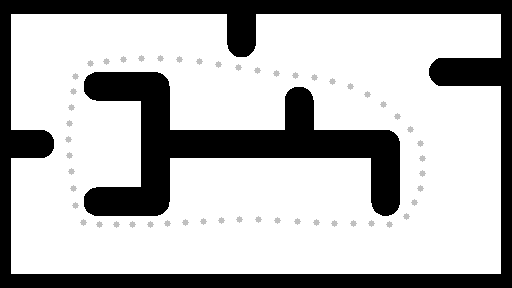
\includegraphics[width=\columnwidth]{snake_result.png}
	\caption[Snake-Ergebnis]{Die resultierenden Kontrollpunkte nach Anwendung des Snake-Algorithmus}
	\label{fig-snake}
\end{figure}

\subsection{Merkmalsberechnung}
Um die Trainingsdauer kurz zu halten und eine möglichst streckenunabhängige KI zu erhalten, wird eine kleine Anzahl aussagekräftiger Merkmale verwendet. Dazu gehören die Geschwindigkeit der Figur, ihre Entfernung zum nächsten Hindernis, sowie ihre Entfernungen zu den nächsten Kontrollpunkten. Im Gegensatz zu der Streckenberechnung, die nur einmalig zu Beginn des Spiels durchgeführt werden muss, müssen diese Merkmale für jeden Frame neu berechnet werden, um sie dem neuronalen Netz als Eingabe zu übergeben und eine Ausgabe zu erhalten.

Da jedes Merkmal auf der aktuellen Position der Figur basiert, ist es wichtig zunächst diese möglichst genau und zuverlässig zu bestimmen. Dazu werden mit einem Schwellenwertverfahren alle Pixel bestimmt, die annähernd die Farbe der gesuchten Figur haben und der Mittelwert über die Positionen aller dieser Pixel gebildet.

Die aktuelle Geschwindigkeit der Figur lässt sich aus der Differenz der aktuellen und der letzten Position berechnen. Dabei wird die Geschwindigkeit in x- und y-Richtung aufgeteilt, stellt also zwei Merkmale dar. Um aber kleinen Störungen und starken Schwankungen der Geschwindigkeit entgegenzuwirken, werden die letzten sieben Positionen der Figur gemerkt und die durchschnittliche Geschwindigkeit in diesem Zeitraum gebildet.

Für die Entfernung zum nächsten Hindernis wird ausgehend von der aktuellen Position berechnet, wie weit das nächste Hindernis in der aktuellen Bewegungsrichtung entfernt ist. Als Hindernisse gelten dabei sowohl die Wände der Strecke als auch gegnerische Figuren.

Um die Entfernungen zu den nächsten Kontrollpunkten zu berechnen, ist es zuerst nötig zu bestimmen, welchem Kontrollpunkt die Figur zur Zeit am nächsten ist. Um dies möglichst schnell herauszufinden, wird bereits zu Beginn des Spiels nach der Streckenerkennung eine Karte angelegt, die jedem Pixel der Strecke ihren nächsten Kontrollpunkt zuordnet. Ist der aktuelle Kontrollpunkt bestimmt, kann durch die Differenz der Position des nächsten Kontrollpunktes und der aktuellen Ballposition die Entfernung in jeweils x- und y-Richtung berechnet werden. Gleiches kann auch für den übernächsten oder weitere Kontrollpunkte unternommen werden, um der KI eine größere Vorausplanung zu ermöglichen.


\section{Experimente und Ergebnisse}

Für die Entwicklung unserer \ac{KI} haben wir verschiedene Parameter unseres Aufbau ausprobiert. Diese Parameter werden nachfolgend vorgestellt. Anschließend werden die ausgewählte Versuche mit ihren Ergebnissen vorgestellt, die zu guten Ergebnissen geführt haben.
Für alle Experimente gilt, das zum Abfahren der geforderten Runden jeweils 3 Minuten Zeit gewesen sind. Die verwendeten \ac{NEAT}-Parameter sind in der Tabelle \ref{tab:NEAT} zu finden.
Zu dem wurden den initialen Population jeweils Kanten mit einer Wahrscheinlichkeit von 0,2 hinzugefügt.
\begin{table}
	\setlength\abovecaptionskip{-0.2\baselineskip}
	\caption{Übersicht der verwendeten \ac{NEAT}-Parameter.}
	\label{tab:NEAT}
	\centering
	\begin{tabular}{|r|c|}
		\hline
		Parameter & Wert \\\hline\hline
		Populationsgröße & 45 \\\hline
		$P\left(\textrm{Knoten hinzufügen}\right)$ & 0,3 \\\hline
		$P\left(\textrm{Knoten entfernen}\right)$ & 0,1 \\\hline
		$P\left(\textrm{Schwellwert-Mutation}\right)$ & 0,8 \\\hline
		$P\left(\textrm{Kante hinzufügen}\right)$ & 0,75 \\\hline
		$P\left(\textrm{Kante entfernen}\right)$ & 0,3 \\\hline
		$P\left(\textrm{Kantengewicht-Mutation}\right)$ & 0,8 \\\hline
		Minimale Anzahl an Spezies & 2 \\\hline
	\end{tabular}
\end{table}
\subsection{Parameter}
\subsubsection*{Anzahl Ausgangsknoten}
Wir haben die \ac{NEAT}-Algorithmus auf zwei verschiedene Ansätze angewendet, wie die Ausgangsneuronen für die Steuerung der Figur interpretiert werden können. 
In dem ersten Ansatz gibt es 4 Ausgangsneuronen, wobei je ein Neuron für eine der Richtungen oben, unten, links oder rechts steht. Da für die Aktivierungsfunktion der Neurone die Sigmoid-Funktion verwendet wurde, kann für ein Ausgangsneuron $o_r$ folgende Interpretation angewendet werden:
\begin{itemize}
	\item $o_r < 0.5:$ Taste $r$ nicht gedrückt
	\item $o_r \geq 0.5:$ Taste $r$ gedrückt.
\end{itemize}
Dabei stet $r$ für die vier verschiedenen möglichen Richtungen.

Für den zweiten Ansatz werden nur zwei Ausgangsneurone $o_h$ und $o_v$ benötigt. Für $o_h$ gilt dabei folgende Interpretation:
\begin{itemize}
	\item $o_h\leq 0.25$: Taste rechts gedrückt
	\item $0.25 < o_h <0.75$: weder Taste links noch Taste rechts gedrückt
	\item $o_h\geq 0.75$: Taste links gedrückt.
\end{itemize}
Für $o_v$ ist die Interpretation analog mit den Richtungen Unten und Oben.

\subsubsection*{Strecke}
Die \acp{KI} wurden entweder ausschließlich auf der ersten Strecke des Spiels oder auf der dritten trainiert.

\subsubsection*{Fitnessfunktion}
Wir haben zwei Arten von Fitnessfunktionen entwickelt. Beide basieren auf den Kontrollpunkten die bei der Streckenerkennung berechnet werden.
Die erste Fitnessfunktion $f_1$ wird über die Anzahl der abgefahrenen Kontrollpunkte definiert:
\begin{equation}
f_1 = \#KP,
\end{equation}
mit $\#KP$ als die Anzahl der abgefahrenen Kontrollpunkte. Die verwendeten Strecken 1 und 3 bestehen aus 48 beziehungsweise 52 Kontrollpunkten.
Die zweite Fitnessfunktion $f_2$ erweitert $f_1$ wie folgt:
\begin{equation}
f_2=\#KP + (180s-t) + 0,25\cdot(255 - s),
\end{equation}
mit $t$ als die benötigte Zeit in Sekunden und $s$ als der erlittene Schaden. Dabei sind 180s und 255 die jeweils maximal möglichen Werte. Die Erweiterung wurde jedoch nur angewendet, wenn das Genome erfolgreich im Ziel angekommen ist, um das Erreichen des Zieles zu belohnen.

\subsubsection*{Kontrollpunkte}
Als letzten Parameter haben wir angegeben, welche Kontrollpunkten als Eingabe verwendet werden. Die Liste $\left[2, 4\right]$ steht zum Beispiel dafür das die Differenzen in x- und y-Richtung von der aktuellen Position zu den übernächsten sowie dem viert nächsten Kontrollpunkt angegeben werden. Pro Kontrollpunkt entstehen also jeweils zwei weitere Eingaben

\subsection{Experimente}
In Tabelle \ref{tab:experimente} sind die jeweiligen Parameter der Experimente dargestellt. Neben den Distanzen zu den jeweiligen Kontrollpunkten wurde die aktuelle Geschwindigkeit in x- und y-Richtung, sowie der Abstand zu dem nächsten Hindernis in der aktuellen Bewegungsrichtung als Eingabe verwendet. Der \ac{NEAT}-Algorithmus wurde auf einer Population der Größe 45 über 200 Generationen angewendet. Um die Laufzeit zu verringern wurde von drei Genomen zur gleichen Zeit der jeweilige Wert der Fitnessfunktion berechnet, indem sie gleichzeitig ein Rennen gefahren sind. Das Genome, das in der 200 Generation den höchsten Wert hat, repräsentiert nachfolgend das jeweilige Experiment.

\begin{table}
	\setlength\abovecaptionskip{-0.4\baselineskip}
	\caption{Übersicht zu den einzelnen Parametern der jeweiligen Experimente.}
	\label{tab:experimente}
	\centering
	\begin{tabular}{|c||c|c|c|c|c|}
		\hline
		Parameter & E1 & E2 & E3 & E4 & E5\\\hline\hline
		\# Ausgangsneurone & 4 & 4 & 2 & 2 & 2\\\hline
		Strecke & 1 & 3 & 3& 3 &3\\\hline
		Fittnessfunktion & $f_1$& $f_1$& $f_1$& $f_2$&$f_2$\\\hline
		Kontrollpunkte & $\left[1\right]$& $\left[2\right]$& $\left[2\right]$& $\left[2\right]$&$\left[2, 4\right]$\\\hline
	\end{tabular}
\end{table}

Nach Anwendung des \ac{NEAT}-Algorithmus, haben wir die Repräsentanten der Experimente in einem Turnier in Zweierduellen gegen einander antreten lassen. In Tabelle \ref{tab:turnier} sind die jeweils benötige Zeit und der erlittene Schaden aus den Duellen zu finden. Dabei wird deutlich, dass das Netz aus Experiment 4 sich gegen alle anderen, im Bezug auf Zeit und Schaden durchsetzen konnte. Daher wird dieses auch in dem Turnier am Ende Projektpraktikums eingesetzt.

\begin{table}
	\setlength\abovecaptionskip{-0.2\baselineskip}
	\caption{Vergleich der Performanz der durch die verschiedenen Experimente generierten Netze.}{Die Zelle in Zeile $n$ und Spalte $m$ enthält die gefahrene Zeit und den erhaltenen Schaden des Netzes $n$ aus dem direkten Vergleich zu Netz $m$. Die letzte Spalte enthält die Durchschnittswerte aus den Duell mit den anderen Netzen, sofern das Duell überlebt wurde. Mit rot, grün und grau, sind jeweils die Niederlagen, Siege oder Unentschieden gekennzeichnet.}
	\label{tab:turnier}
	\centering
	\begin{tabular}{|c|c|c|c|c|c|c|}
		\hline
		& E1                                                   & E2                            & E3                            & E4                            & E5                            & Durchschnitt \\ \hline
		& \cellcolor[HTML]{C0C0C0} 3:17 & \cellcolor[HTML]{C0C0C0}3:24 & \cellcolor[HTML]{FFCCC9}3:29 & \cellcolor[HTML]{FFCCC9}2:47 & \cellcolor[HTML]{FFCCC9}3:05 & \cellcolor[HTML]{C0C0C0}-       \\ \cline{2-7} 
		\multirow{-2}{*}{E1} & \cellcolor[HTML]{C0C0C0}255 & \cellcolor[HTML]{C0C0C0}255  & \cellcolor[HTML]{FFCCC9}255  & \cellcolor[HTML]{FFCCC9}255  & \cellcolor[HTML]{FFCCC9}255  & \cellcolor[HTML]{C0C0C0}255     \\ \hline
		& \cellcolor[HTML]{C0C0C0}2:02                        & \cellcolor[HTML]{C0C0C0}2:23 & \cellcolor[HTML]{FFCCC9}2:31 & \cellcolor[HTML]{FFCCC9}2:17 & \cellcolor[HTML]{FFCCC9}2:18 & \cellcolor[HTML]{C0C0C0}-       \\ \cline{2-7} 
		\multirow{-2}{*}{E2} & \cellcolor[HTML]{C0C0C0}255                         & \cellcolor[HTML]{C0C0C0}255  & \cellcolor[HTML]{FFCCC9}255  & \cellcolor[HTML]{FFCCC9}255  & \cellcolor[HTML]{FFCCC9}255  & \cellcolor[HTML]{C0C0C0}255     \\ \hline
		& \cellcolor[HTML]{9AFF99}3:23                        & \cellcolor[HTML]{9AFF99}3:22 & \cellcolor[HTML]{C0C0C0}3:10 & \cellcolor[HTML]{FFCCC9}3:20 & \cellcolor[HTML]{FFCCC9}3:30 & \cellcolor[HTML]{C0C0C0}3:24    \\ \cline{2-7} 
		\multirow{-2}{*}{E3} & \cellcolor[HTML]{9AFF99}160                         & \cellcolor[HTML]{9AFF99}76   & \cellcolor[HTML]{C0C0C0}56   & \cellcolor[HTML]{FFCCC9}146  & \cellcolor[HTML]{FFCCC9}162  & \cellcolor[HTML]{C0C0C0}136     \\ \hline
		& \cellcolor[HTML]{9AFF99}3:11                        & \cellcolor[HTML]{9AFF99}3:20 & \cellcolor[HTML]{9AFF99}3:19 & \cellcolor[HTML]{C0C0C0}3:13 & \cellcolor[HTML]{9AFF99}3:16 & \cellcolor[HTML]{9AFF99}3:17    \\ \cline{2-7} 
		\multirow{-2}{*}{E4} & \cellcolor[HTML]{9AFF99}92                          & \cellcolor[HTML]{9AFF99}120  & \cellcolor[HTML]{9AFF99}129  & \cellcolor[HTML]{C0C0C0}70   & \cellcolor[HTML]{9AFF99}102  & \cellcolor[HTML]{9AFF99}110,75  \\ \hline
		& \cellcolor[HTML]{9AFF99}3:16                        & \cellcolor[HTML]{9AFF99}3:19 & \cellcolor[HTML]{9AFF99}3:18 & \cellcolor[HTML]{FFCCC9}3:19 & \cellcolor[HTML]{C0C0C0}3:17 & \cellcolor[HTML]{C0C0C0}3:18    \\ \cline{2-7} 
		\multirow{-2}{*}{E5} & \cellcolor[HTML]{9AFF99}116                         & \cellcolor[HTML]{9AFF99}131  & \cellcolor[HTML]{9AFF99}144  & \cellcolor[HTML]{FFCCC9}174  & \cellcolor[HTML]{C0C0C0}117  & \cellcolor[HTML]{C0C0C0}141,25  \\ \hline 
	\end{tabular}
\end{table}

\begin{figure}
	\centering
	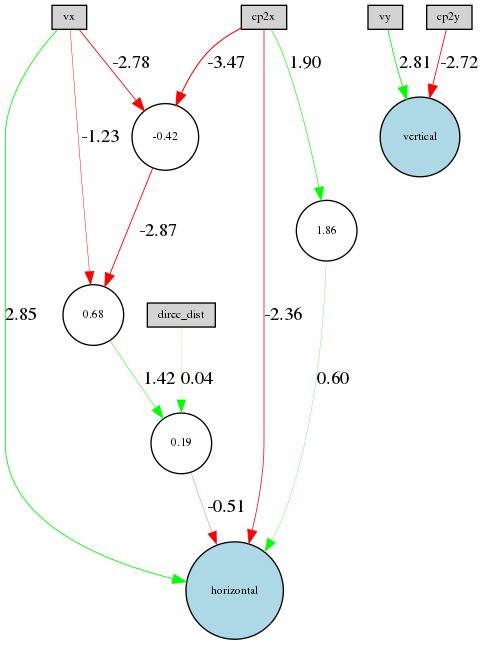
\includegraphics[height=250px]{winner_e4_clean.png}
	\caption{Das neuronale Netz des Repräsentanten des Experiment 4. Aus Gründen der Übersichtlichkeit wurden deaktivierte Kanten, sowie Knoten und Kanten, von den man die Ausgangsknoten nicht erreichen kann, nicht dargestellt}
	\label{fig:netz}
\end{figure}

In Abbildung \ref{fig:netz} ist das neuronal Netz aus Experiment 4 dargestellt. Dabei ist auffällig, dass für die vertikale Steuerung ein lineares Modell, basierend auf der vertikalen Geschwindigkeit und der vertikalen Abweichung zum Kontorotrollpunkt vorliegt. Für den horizontalen Fall ist das nicht ganz gegeben, wobei die zusätzlichen Kanten und Knoten nur einen vergleichsweise geringen Einfluss auf die Ausgabe habe. Auch in anderen Experimenten konnte die Bildung eines linearen Modells beobachtet werden.

Aus dem Vergleich den Experimente lassen sich die Vermutungen aufstellen, dass zum einen die Wahl von zwei Ausgangsknoten zu besseren Ergebnissen führt, da ein einfacheres Modell gelernt werden muss. Zum anderen kann die erweiterte Fitnessfunktion $f_2$ dazu führen, dass die Genome ein etwas schnelleres und sicheres Fahren lernen. Die Wahl von mehreren Kontrollpunkten erschwert das Problem. Allerdings könnten über mehr Generationen auch bessere Ergebnisse erzielt werden. Diese Vermutungen müssten noch durch intensivere Untersuchengen bestätigt werden.

\section{Zusammenfassung}
Wir haben im Rahmen des Praktikums mithilfe von Streckenerkennung, Merkmalsberechnung und dem \ac{NEAT}-Algorithmus mehrere \acp{KI} für das Spiel rAIcer entwickelt. Diese haben wir mit einander verglichen. Das beste Netz wurde mit 2 Ausgangsneuronen, der erweiterten Fitnessfunktion und mit einem Kontrollpunkt entwickelt. Dieses Netz ist in der Lage auf den bereitgestellten Strecken das Ziel zu erreichen. Überraschen ist, das durch \ac{NEAT} stellen weise sehr einfache Modelle für die Steuerung gelernt werden.
\bibliography{Quellen}{}
\bibliographystyle{./IEEEtranBST2/IEEEtran}
\end{document}